96. \begin{figure}[ht!]
\center{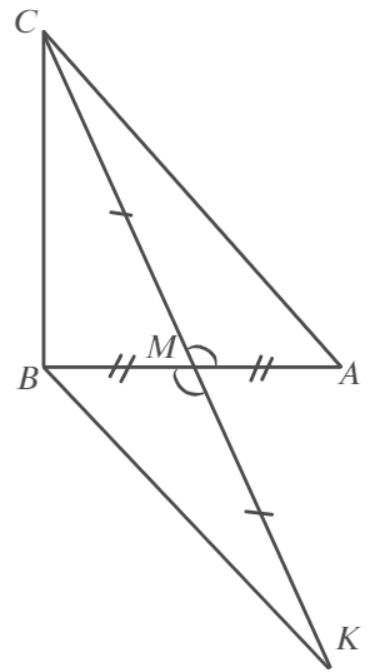
\includegraphics[scale=0.35]{g96.png}}
\end{figure}\\
Пусть $\angle A=3x,\ \angle B=5x,\ \angle C=2x,$ тогда $3x+5x+2x=180^\circ,\ 10x=180^\circ,\ x=18^\circ.$ Тогда $\angle A=3\cdot18^\circ=54^\circ.$
$\left.\begin{array}{l}CM=MK,\\
BM=MA,\\
\angle CMA=\angle BMK\text{ (вертикальные).}\end{array}\right\}\Rightarrow \Delta CMA=\Delta KMB\text{ по I признаку}\Rightarrow \angle ABK=\angle MBK=\angle A=54^\circ.$\newpage
\noindent97. \begin{figure}[ht!]
\center{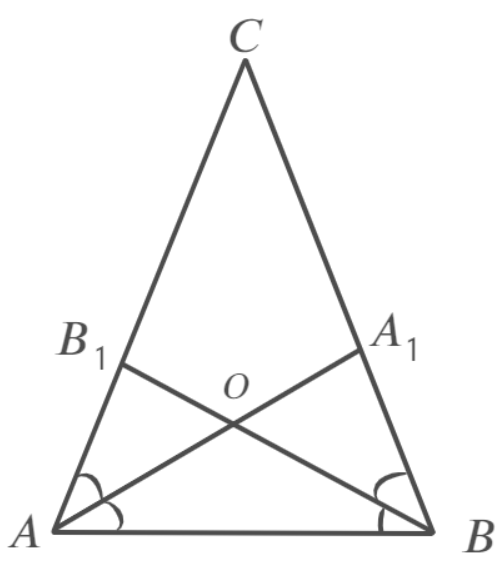
\includegraphics[scale=0.35]{g97.png}}
\end{figure}\\
Пусть $\angle A=\angle B=x,\ \angle C=180^\circ-2x.$ Тогда возможны два случая: $x+30^\circ=180^\circ-2x,\ 3x=150^\circ,\ x=50^\circ$ или $x-30^\circ=180^\circ-2x,\
3x=210^\circ,\ x=70^\circ.$ В первом случае  $\angle B_1AO=50^\circ:2=25^\circ,\ \angle AB_1O=180^\circ-3\cdot25^\circ=105^\circ,\ \angle AOB_1=180^\circ-25^\circ-105^\circ=50^\circ.$ Во втором случае  $\angle B_1AO=70^\circ:2=35^\circ,\ \angle AB_1O=180^\circ-3\cdot35^\circ=75^\circ,\ \angle AOB_1=180^\circ-35^\circ-75^\circ=70^\circ.$\\
